\begin{center}

  \begin{tabular}{rp{16cm}lp{20cm}}%{rl}

  % after \\: \hline or \cline{col1-col2} \cline{col3-col4} ...

  论文地址:& \href{https://ieeexplore.ieee.org/stamp/stamp.jsp?tp=\&arnumber=7780459}{https://ieeexplore.ieee.org/stamp/stamp.jsp?tp=\&arnumber=7780459} \\
  来源:& CVPR, 2016\\
  作者:& Kaiming He Xiangyu Zhang, et al. \\

  源码:& \href{https://github.com/KaimingHe/deep-residual-networks}{deep-residual-networks} \\

%  slides:& \href{http://yunshengb.com/wp-content/uploads/2017/03/nips_2018_r2l_workshop_talk.pdf}{{\footnotesize Convolutional Set Matching for Graph Similarity}}\\

  关键词:& \textbf{Residual Learning, Shortcut Connection} \\

  写于:& \date{2021-03-15}

  \end{tabular}

\end{center}

该论文\cite{he2016deep}主要解决的深层神经网络的训练问题。随着网络的深度的增加,模型的效果反而变差了,论文提出了Residual Learning的方式来训练深层的神经网络。

\paragraph{问题定义}
基于深度神经网络模型在图像领域的很多任务上都取得了重大的突破,其中模型的深度起到了关键性的作用。但是随着模型深度的增加,一系列问题出现了:\textbf{深度的模型只是堆叠更多的层就可以了吗?}随着层数的增加,会出现梯度消失/爆炸问题,这个问题可以通过不同的归一化来解决。但还有一个问题:degradation --- 模型退化。Degradation是论文解决的问题。那么什么是模型退化呢?
\begin{figure}[h]
	\centering
	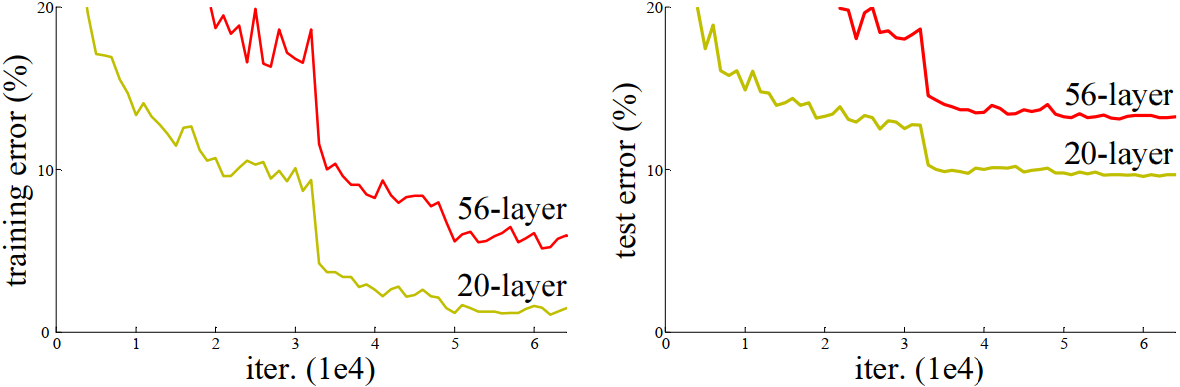
\includegraphics[width=.5\textwidth]{pics/degradation.png}
	\caption{Degradation}
	\label{fig:degradation}
\end{figure}

考虑一个已经训练好的模型,它能达到一定的效果,为了让效果更好,我们在训练好的模型的基础上增加层,再进行训练。按照常理,新增的层就算学习到了恒等映射模型也不会退化的,但是一些实验显示,增加层后的模型的效果不但没有提升反而还下降了!\textbf{模型退化}了!这表明:\tbc{red}{在求解时,使用多个非线性层来近似恒等映射可能是比较困难的}。

\paragraph{Residual Learning}

\begin{figure}[h]
	\centering
	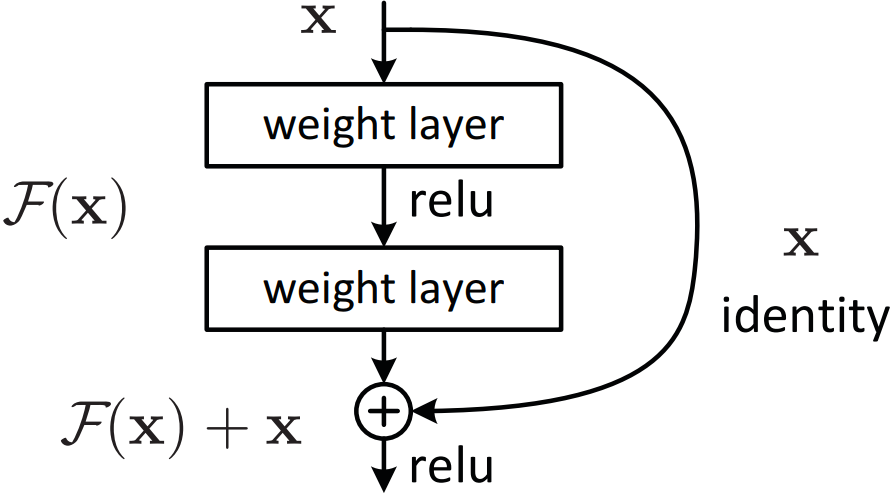
\includegraphics[width=.4\textwidth]{pics/residual.png}
	\caption{Residual learning: a building block}
	\label{fig:residual}
\end{figure}
为了解决模型退化的问题,作者提出了\textit{deep residual learning} framework。
在加深模型时,我们通常希望新加的层能够直接学习到潜在的映射函数$\mathcal{H}(x)$,residual learning并不是如此,而是学习一个residual mapping $\mathcal{F}(x) = \mathcal{H}(x) - x$。那么原来期望学习到的映射就可以表示成:$\mathcal{H}(x) = \mathcal{F}(x) + x$。这里有一个假设:\textbf{$\mathcal{F}$比$\mathcal{H}$更容易优化}。

$\mathcal{F}(x) + x$可以用一个带有shortcut连接的前馈神经网络模拟,如Fig.\ref{fig:residual}所示。如果恒等映射是最优解,那么只需要使residual block中层的参数为零即可。结合之前所说的非线性层难以学习identity,residual block不仅包含了identity部分,还包括了非线性部分,这样的一个映射不仅可以学习到复杂的非线性部分,还可以学习到非线性层难以学习到的线性部分(不仅是identity,还可以是$ax+b$,线性函数加非线性函数)。

Fig.\ref{fig:residual}所示的残差块可以表示为:
$$
\mathbf{y}=\mathcal{F}\left(\mathbf{x},\left\{W_{i}\right\}\right)+  \mathbf{x}
$$
\begin{center}
	或
\end{center}
$$
\mathbf{y}=\mathcal{F}\left(\mathbf{x},\left\{W_{i}\right\}\right)+W_{s} \mathbf{x}
$$
以两层的残差块为例,$\mathcal{F}(x, {W_i}) = W_2\sigma (W_1 x)$表示需要学习的残差函数。当然,除了Fig.\ref{fig:residual}所示的残差块,还可以有三层甚至更多层的残差块。论文中还对shortcut connection的形式进行了实验验证,第二种形式的形式效果可能会稍微好一点点,但是可以忽略,而identity形式的残差具有更少的参数、更低的复杂度。


\paragraph{方法的问题/优势}

\begin{itemize}

	\item 研究深度模型中的退化问题,累积的非线性层可能难以学习到线性映射
	\item 提出了residual learning,助力深度模型的学习,且没有增加学习的参数
	\item 提出了ResNet

\end{itemize}


\paragraph{方法的局限性/未来方向}

\begin{itemize}

	\item 累加的非线性层可能可以学习到较复杂的非线性变化,但是难以通过非线性层学习到线性变换,residual learning弥补了这一缺点
	

\end{itemize}